\section{Models}

In this section we will present the different types of models that we will later train during the experiments. 

\subsection{Methodology}
% how did we proceed to select types of models to train
For the set of models that we chose to train in this project, we will apply the same methodology. First, the dataset over which we want to train the model will be split into a training and a testing set, by using random sampling with a proportion of 70\% individuals in the training and 30\% individuals in the testing set. Then the model will be trained over the training set by using k-fold cross validation, to select the best hyper parameter values for the model. After selecting the best hyper parameters, the model will be trained with those parameters over the whole training set. Finally, the trained model will be used to predict over the testing set to extract error measures and see how well the model generalizes.\\
In order to be able to compare over all the selected best models of each type, we will make sure that we extract the same error measure. In this case, we will use the normalized root mean squared error (NRMSE).

\subsection{Model types}
\textbf{Linear} We used the Linear model as the baseline to our exploration. This model has no control over the complexity so it is expected to overfit and perform worse than the other models overall.

\textbf{Ridge regression} This is one the most famous regularized linear models, using the L2 norm. It has a great support in libraries, with many implementations.

\textbf{Lasso regression}
This is another well-known regularized linear model, this one using the L1 norm. 

\textbf{PCR} This model is taking advantage of the PCA and use it to predict. First, the model will create PCA transformation over the training data, then we need to decide the number of PCs we want to use, we choose PCs' that will explain at least $90\%$ of the variance in the data. Later we predict using those PCs.

\textbf{Decision trees} We need to find tree that will give us good prediction but we don't want to have huge tree, therefore we needed to prune the tree using the complexity parameter. In first step we build a tree with cross-validation parameter of 10. Given full tree from the library we wish to prune it. We check the CV error of the best offer given tree (mostly it was the biggest tree the model created). To the CV error we added it's SD error, by that we get an interval of error for the best tree. Our next step is to choose the smallest tree that it's CV error is in that range. By prune the tree to that size we ensure that we will not have a complex tree and yet our CV error will be in the CV error range of the best tree this model can offer. One very important advantage of the tree is the ability to interpreted its decision. However,  since we don't do classification, it will get the centeroid of the leaf. In Figure.\ref{fig:dt},\ref{fig:dtp} we can see example of tree before and after pruning base on the initial dataset.

\begin{multicols}{2}
\begin{figure}[H]
\centering
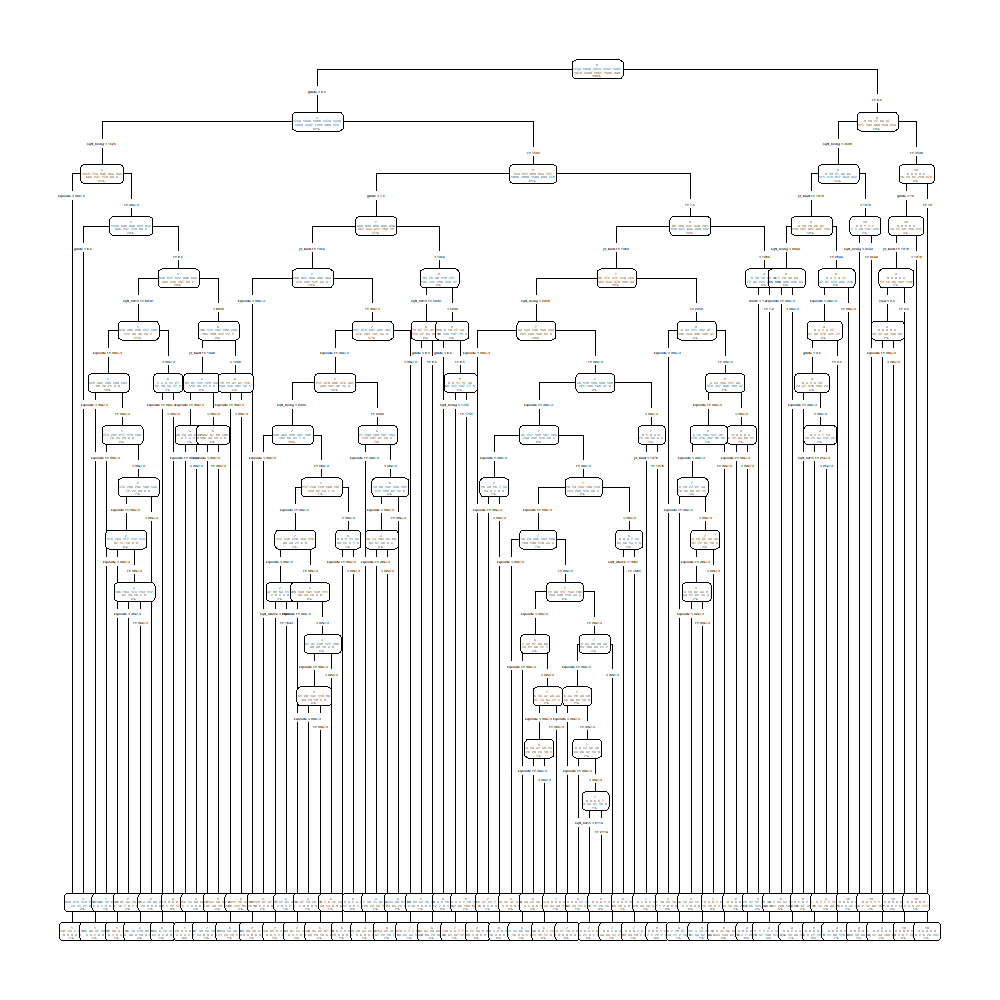
\includegraphics[width=0.48\textwidth]{img/trainingdt.png}
\caption{Full decision tree}
\label{fig:dt}
\end{figure}
\begin{figure}[H]
\centering
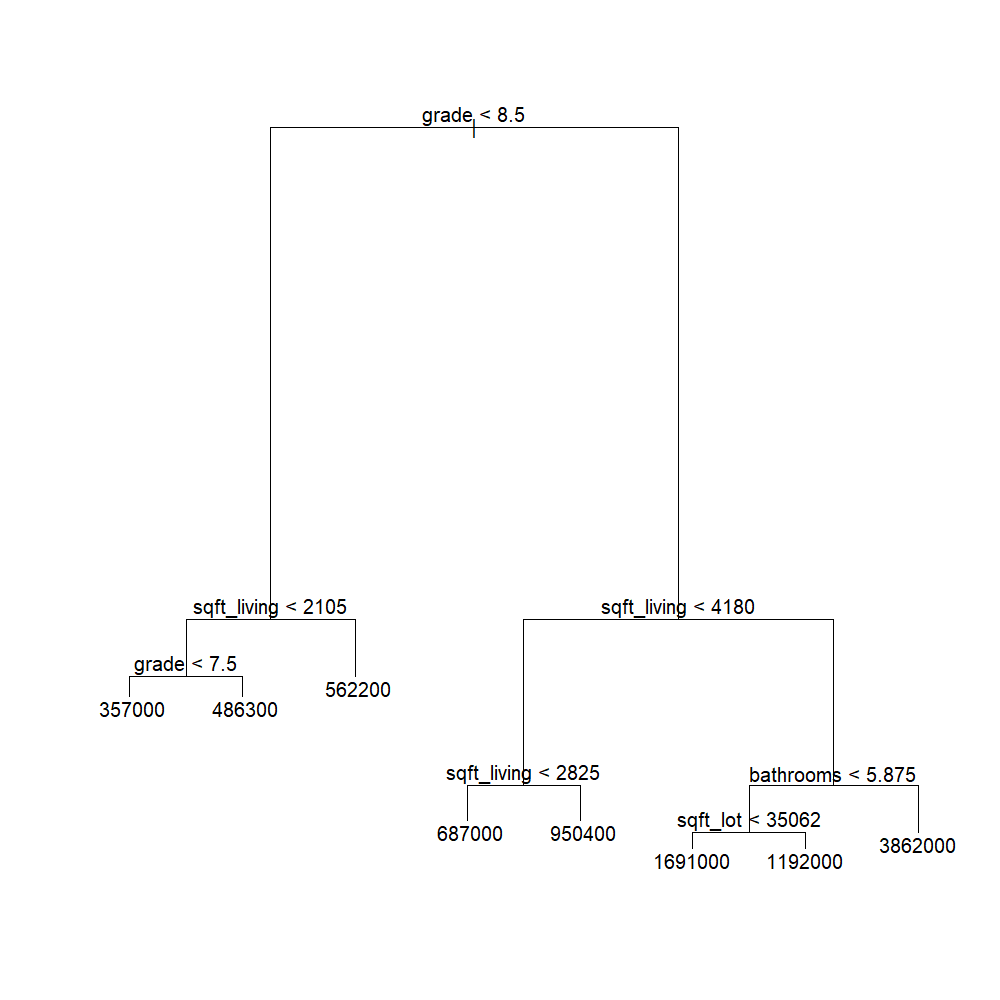
\includegraphics[width=0.48\textwidth]{img/regression_treelib_tree_training.png}
\caption{Prune decision tree}
\label{fig:dtp}
\end{figure}
\end{multicols}


\textbf{Random Forest} We need to find the optimum number of trees to generate. We do that using the MSE of the validatiion error. We train and validate number of models with over  different number of trees, then, we choose the model that have the minimum MSE. The next step was to train the model using the whole training data and predict. We use RandomForest R library.

